% Graphics for slide 12, in the order the PDF draws them.
\begin{tikzpicture}[remember picture, overlay, x=1bp, y=-1bp,
  shift={(current page.north west)}]
\path[fill=cFFFFFF] (0,0) rectangle (960,540);
\node[anchor=north west, inner sep=0pt] at (56.69,477.21) {
\includegraphics[width=73.42bp, height=37.42bp]{figures/fundamentals-of-hpc/p03-1.png}};
\path[fill=cEE7628,even odd rule] (57.18,55.73) ..controls(57.96,55.73)and(58.6,56.37)..(58.6,57.15) --(58.6,85.5) ..controls(58.6,86.28)and(57.96,86.91)..(57.18,86.91) ..controls(56.4,86.91)and(55.76,86.28)..(55.76,85.5) --(55.76,57.15) ..controls(55.76,56.37)and(56.4,55.73)..(57.18,55.73);
\node[anchor=north west, inner sep=0pt] at (195.78,118.02) {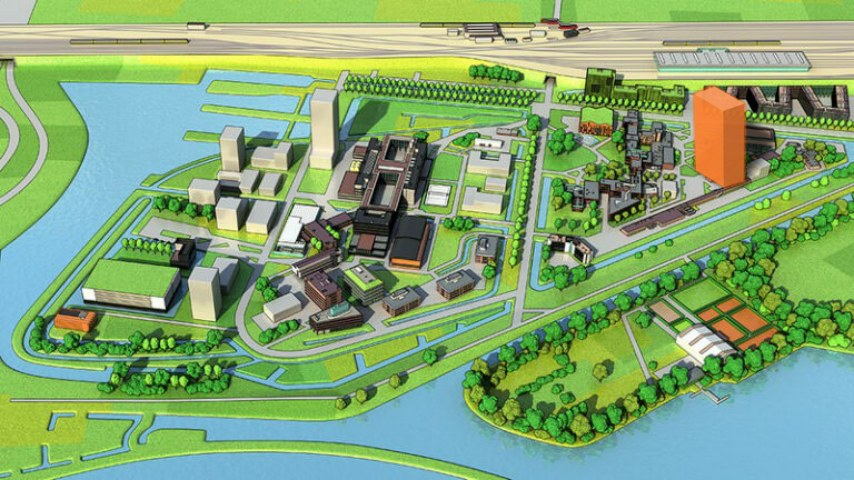
\includegraphics[width=568.44bp, height=319.75bp]{figures/fundamentals-of-hpc/p12-2.jpg}};
\node[anchor=north west, inner sep=0pt] at (648.84,159.36) {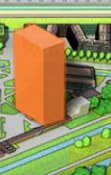
\includegraphics[width=73.44bp, height=116.4bp]{figures/fundamentals-of-hpc/p12-3.jpg}};
\path[fill=cEE7628,even odd rule] (653.58,280.23) ..controls(653.58,277.62)and(655.69,275.51)..(658.3,275.51) --(766.6,275.51) ..controls(769.21,275.51)and(771.32,277.62)..(771.32,280.23) --(771.32,299.11) ..controls(771.32,301.72)and(769.21,303.83)..(766.6,303.83) --(658.3,303.83) ..controls(655.69,303.83)and(653.58,301.72)..(653.58,299.11) --(653.58,280.23);
\path[draw=cEE7628,line width=3bp] (685.07,240.38) --(712.45,275.5);
\path[fill=cEE7628,even odd rule] (504.95,345.69) ..controls(504.95,343.08)and(507.06,340.97)..(509.67,340.97) --(579.37,340.97) ..controls(581.97,340.97)and(584.09,343.08)..(584.09,345.69) --(584.09,364.57) ..controls(584.09,367.18)and(581.97,369.29)..(579.37,369.29) --(509.67,369.29) ..controls(507.06,369.29)and(504.95,367.18)..(504.95,364.57) --(504.95,345.69);
\path[draw=cEE7628,line width=3bp] (544.52,340.97) --(573.91,288.18);
\path[fill=cEE7628,even odd rule] (410.51,374.56) ..controls(410.51,371.95)and(412.62,369.83)..(415.23,369.83) --(493.13,369.83) ..controls(495.74,369.83)and(497.85,371.95)..(497.85,374.56) --(497.85,393.44) ..controls(497.85,396.05)and(495.74,398.16)..(493.13,398.16) --(415.23,398.16) ..controls(412.62,398.16)and(410.51,396.05)..(410.51,393.44) --(410.51,374.56);
\path[fill=cEE7628,even odd rule] (325.01,151.62) ..controls(325.01,149.01)and(327.13,146.9)..(329.73,146.9) --(407.64,146.9) ..controls(410.24,146.9)and(412.36,149.01)..(412.36,151.62) --(412.36,170.51) ..controls(412.36,173.11)and(410.24,175.23)..(407.64,175.23) --(329.73,175.23) ..controls(327.13,175.23)and(325.01,173.11)..(325.01,170.51) --(325.01,151.62);
\path[draw=cEE7628,line width=3bp] (368.69,175.23) --(449.51,244.72);
\path[draw=cEE7628,line width=3bp] (454.18,369.83) --(492.52,316.78);
\end{tikzpicture}
